\documentclass[11pt]{article}

\usepackage[margin=1.0in]{geometry}
%\linespread{1.5}
\usepackage{graphicx}
\usepackage{amsmath}
\usepackage{cite}

% definition of \customlabel, which is used to label supplementary figures and tables
\makeatletter
\newcommand{\customlabel}[2]{%
\protected@write \@auxout {}{\string \newlabel {#1}{{#2}{\thepage}{}{}{}}}}
\makeatother



\renewcommand{\bottomfraction}{.9}
\renewcommand{\topfraction}{.9}
\renewcommand{\textfraction}{0.1}
\renewcommand{\floatpagefraction}{.9}


\begin{document}

\section*{Introduction}

Over the years, various methods have been used to calculate the strength of natural selection acting on protein-coding sequences. Traditionally, the focus has been on estimating the evolutionary rate ratio, $dN/dS$, the rate of nonsynonymous to synonymous substitution rates. This metric indicates how quickly a protein's constituent amino acids change, and is widely used to identify cases of positive selection ($dN/dS > 1$). Following early counting methods for estimating $dN/dS$ (e.g. refs \cite{LWL85} and \cite{NG86}), mechanistic codon substitution models, which assume an explicit Markov-process model of sequence evolution (see ref.~\cite{Anisimova2009} for a comprehensive review), have taken a leading role as the inferenqce method of choice since their introduction in the 1990s \cite{GoldmanYang1994, MuseGaut1994, NielsenYang1998}. These models yield maximum likelihood estimates (MLEs) for the parameter $\omega$, which represents the quantity $dN/dS$, and have seen great success in the field of molecular evolution. 

A second class of models, known as mutation-selection-balance (MutSel) models, has emerged recently as a popular alternative to mechanistic codon models. The MutSel framework, couched firmly in population genetics theory, models the dynamic interplay between mutation and selection in a protein-coding sequence. MutSel models yield estimates of site-wise scaled selection coefficients, which indicate the extent to which natural selection favors, or disfavors, particular codons or amino acids at a given protein position. Although MutSel models were first introduced over 15 years ago \cite{HalpernBruno1998}, they have seen virtually no use due to their high computational expense. However, recently, several computationally tractable model implementations have emerged \cite{RodrigueLartillot2014,Tamurietal2014}, allowing for the first time the potential for widespread use. 

Although both $dN/dS$ models and MutSel models describe the same fundamental process of protein-coding sequence evolution along a phylogeny, it is largely unknown how these two classes of models relate to one another. In particular, as these inference methods have been developed independently, it remains an open question whether or not parameter estimates from one model are comparable to those of the other model. Therefore, while certain rhetorical arguments may be made in favor of using one method over another, there is currently no formalized, concrete rationale to guide researchers in their methodological choices. 

Here, we formalize the relationship between $\omega$ and MutSel models by examining the extent to which their focal parameters, $dN/dS$ and scaled selection coefficients, yield overlapping information about the evolutionary process. To this end, we derive a mathematical relationship these models' primary parameters from which one can infer $dN/dS$ values from selection coefficients alone. Using a simulation approach, we verify that $dN/dS$ values estimated using selection coefficients alone correspond precisely to $\omega$ MLEs inferred using standard mechanistic codon models. 

(???)Further, we prove that, under conditions of symmetric mutation rates, this relationship holds only under regimes of purifying selection or neutral evolution ($dN/dS \leq 1$). This proof reveals that MutSel models are inherently unable to describe accurately protein evolution under a regime of positive diversifying selection, or when $dN/dS > 1$.

Moreover, our analyses incidentally have revealed certain biases inherent in the ML $\omega$ inference approach. (...)
 


\section*{Methods}

\subsection*{Sequence simulation}
We simulated protein-coding sequences as a continuous-time Markov
process \cite{Yang2006} according to the MutSel model proposed by \cite{HalpernBruno1998}. This model's instantaneous rate matrix $Q$ is given by 

\begin{equation}
Q_{ij} = \left\{ \begin{array}{rl}
              f_{ij}\mu_{ij}\kappa               &\mbox{single nucleotide transition} \\
              f_{ij}\mu_{ij}                          &\mbox{single nucleotide transversion} \\
              0                                           &\mbox{multiple nucleotide changes} \\             
         \end{array} \right.,
\end{equation} where $\mu_{ij}$ is the symmetric nucleotide mutation rate and $f_{ij}$, the fixation probability from codon $i$ to $j$, is defined as \begin{equation}f_{ij} = ln\bigg{(}\frac{\pi_j\mu_{ij}}{\pi_i\mu_{ji}}\bigg{)}\bigg{/}\bigg{(}1 - \frac{\pi_i\mu_{ji}}{\pi_j\mu_{ij}}\bigg{)},\end{equation} where $\pi_i$ is the equilibrium frequency of codon $i$.

We simulated protein-coding sequences along a 10-taxon phylogeny, with all branch lengths equal to 0.01, beginning with a root sequence selected using steady-state codon frequencies. All simulations featured a symmetric mutation rate $\mu_{xy} = 10^{-6}$, and a value for for $\kappa$ was drawn from $\mathcal{U} \sim (1,6)$, resulting in a fully symmetric mutation matrix. Unless otherwise stated, all simulated alignments contained 500,000 codon positions. A single evolutionary model was applied to all positions in the simulated sequences. While this lack of site-wise heterogeneity is unrealistic for real sequence evolution, it allows us to verify our derived relationship between selection coefficients and $dN/dS$ with a sufficiently sized data set.

\subsection*{Assigning scaled selection coefficients}

We simulated 100 alignments under the assumption that all synonymous codons have equal fitness (e.g. no codon bias), and a second set of 100 alignments which incorporated codon bias. For both frameworks, we generated amino acid scaled selection coefficients, $S_a$, for each simulation, by fixing one coefficient to 0 and drawing the remaining 19 values from a normal distribution $\mathcal(N)\sim(0,x)$, where $x \sim U(1,2)$. 

For simulations with no codon bias, we assigned these coefficients to codons such that all synonymous codons had the same scaled selection coefficient. For simulations with codon bias, we randomly selected, for each set of synonymous codons, a preferred codon and designated the rest non-preferred. We then assigned the preferred codon a selection coefficient of $S_a + x$, where $x=ln(2)$, and we assigned non-preferred codons selection coefficients of $S_a - x/(k-1)$, where $k$ is the total number of synonymous codons for the given amino acid. In this way, the average selection coefficient for this amino acid remained unchanged, whereas selective strength was partitioned such that a single codon was preferred.



\subsection*{$dN/dS$ Inference}
We calculated a global $dN/dS$ for each alignment using the mathematical framework outlined in \eqref{eq:pi_i}--\eqref{eq:dS} as well using standard maximum likelihood methods. Specifically, we estimated the $\omega$ parameter using the M0 mechanistic codon model\cite{Yangetal2000}, as implemented in HyPhy \cite{KosakovskyPondetal2005}. We used the GY94 instantaneous rate matrix \cite{GoldmanYang1994,NielsenYang1998}, which includes the primary parameters $\omega$, $\kappa$, and equilibrium codon frequencies. As different $\kappa$ and equilibrium codon frequency parameterizations can change $\omega$ estimates \cite{YN00, Yang2006, ZhangYu2006}, we inferred $\omega$ under a variety of model parameterizations, including three $\kappa$ parameterizations ($\kappa$ fixed to 1, $\kappa$ as a free parameter, and $\kappa$ fixed to its true, simulated value), and four codon frequency specifications (equal codon frequencies,  F3x4 codon frequencies \cite{MuseGaut1994}, CF3x4 codon frequencies \cite{Pond2010} and empirical codon frequencies). These different specifications yielded twelve $\omega$ MLEs per simulated alignment. Note that we additionally verified that the system was evolving under a state-state process by verifying that the true, simulated codon frequencies were the same as the empirical codon frequencies calculated from the simulated alignment. All code used is freely available at \textbf{github}. 



\section*{Results}


\section*{Mathematical relationship between selection coefficients and omega}


We describe here how to calculate $dN/dS$ from the parameters of a MutSel model. Under the assumption that the mutational process is symmetric, e.g. $\mu_{xy}=\mu_{yx}$ for all nucleotide pairs $xy$, we can write the steady-state frequency of codon $i$ as 
\begin{equation}\label{eq:pi_i}
 \pi_i=\frac{e^{S_i}}{\sum_k e^{S_k}},
\end{equation}
where the sum in the denominator runs over all 61 sense codons \cite{SellaHirsh2005}. Here, $S_i$ is the scaled selection coefficient for codon $i$; larger $S_i$ values correspond to higher frequencies of codon $i$.

The fixation probability for a mutation from codon $i$ to codon $j$ is \cite{HalpernBruno1998,SellaHirsh2005}
\begin{equation}\label{eq:f_ij}
 f_{ij} = \frac{1-(\pi_i/\pi_j)^{1/N_e}}{1-\pi_i/\pi_j}
  \approx \frac{1}{N_e} \frac{\ln \pi_j - \ln \pi_i}{1-\pi_i/\pi_j}\,,
\end{equation}
where $N_e$ is the effective population size. Using this framework, we can calculate an evolutionary rate by summing over all substitution probabilities weighted by the frequency of the originating codon. Further, we can establish specific expressions for nonsynonymous and synonymous evolutionary rates, and then divide them in order to obtain a value for the evolutionary rate ratio $dN/dS$.

To begin, we can write the nonsynonymous rate $K_\text{N}$ as 
\begin{equation}\label{eq:KN}
  K_\text{N} = N_e \sum_i \sum_{j \in {\cal N}_i} \pi_i  f_{ij}\mu_{ij}\,,
\end{equation}
where ${\cal N}_i$ is the set of codons that are nonsynonymous to codon $i$ and differ from it by one nucleotide. To normalize $K_\text{N}$, we divide it by the number of nonsynonymous sites, which we calculate according to the mutational opportunity definition of a site \cite{GoldmanYang1994, Yang2006} as 
\begin{equation}\label{eq:LN}
  L_\text{N} = \sum_i \sum_{j \in {\cal N}_i} \pi_i \mu_{ij}\,, 
\end{equation} and thus we find that 
\begin{equation}\label{eq:dN}
  dN = \frac{K_\text{N}}{L_\text{N}}=\frac{ N_e \sum_i \sum_{j \in {\cal N}_i} \pi_i f_{ij} \mu_{ij} } {\sum_i \sum_{j \in {\cal N}_i} \pi_i \mu_{ij} }\,.
\end{equation}

Similarly, for $dS$, the synonymous evolutionary rate $K_\text{S}$ per synonymous site $L_\text{S}$, we find
\begin{equation}\label{eq:dS}
  dS = \frac{K_\text{S}}{L_\text{S}}=\frac{ N_e \sum_i \sum_{j \in {\cal S}_i} \pi_i f_{ij} \mu_{ij} } {\sum_i \sum_{j \in {\cal S}_i} \pi_i \mu_{ij} }\,,
\end{equation}
where ${\cal S}_i$ is the set of codons that are synonymous to codon $i$ and differ from it by one nucleotide substitution. The quantities $K_\text{S}$ and $L_\text{S}$ are defined as in Eqs.~\eqref{eq:KN} and \eqref{eq:LN} but summing over $j\in {\cal S}_i$ instead of $j\in {\cal N}_i$.

Equations \eqref{eq:pi_i}--\eqref{eq:dS} establish a connection between the scaled selection coefficients and the evolutionary rate ratio $dN/dS$. Moreover, we note that, if we assume that all synonymous codons have equal fitness (e.g. synonymous mutations are neutral), the synonymous fixation rate $f_ij = 1/N_e$ \cite{CrowKimura1970}. Under this circumstance, the value for $dS$ would reduce to 1.


\subsection*{Scaled selection coefficients fully encapsulate $\omega$}

To validate our derived relationship between scaled selection coefficients and $dN/dS$, we simulated protein-coding sequences along a 10-taxon phylogeny according to a mutation-selection model framework \cite{HalpernBruno1998,SellaHirsh2005}. We simulated 100 alignments which gave equal fitness values to synonymous codons, and 100 alignments which incorporated codon bias (see Method for details). All simulations assumed a symmetric nucleotide rate matrix. For each alignment, we calculated $dN/dS$ using equations \eqref{eq:pi_i}--\eqref{eq:dS} as well as using the M0 mechanistic codon model \cite{GoldmanYang1994,NielsenYang1998,Yangetal2000} rate matrix, as implemented in the HyPhy batch language \cite{KosakovskyPondetal2005}.

As shown in Figure~\ref{reg_conv}A, $dN/dS$ values derived using selection coefficients agree nearly perfectly with those inferred using standard maximum likelihood methods. We additionally demonstrate convergence of these values with increasing amounts of data, represented by simulated alignment length (Figure~\ref{reg_conv}B). Taken together, these results clearly show that MutSel model parameters fully encapsulate information regarding $dN/dS$, and that the results from MutSel and $\omega$ models are in complete agreement. 

Moreover, as seen in Figure~\ref{reg_conv}A, $dN/dS$ values are always less than 1, reflecting a universal regime of purifying selection. In fact, \textbf{in SuppMat,} we prove that, when calculated using scaled selection coefficients, $dN/dS$ is necessarily always less than or equal to 1. This important insight reveals that, while MutSel and mechanistic codon models fully agree, their relationship only holds under conditions of purifying selection or neutral evolution. MutSel models, therefore, are inherently unable to describe protein evolution under positive, diversifying selection ($dN/dS > 1$).

BUT NOTE ABOUT THE SYNONYMOUS FITNESS DIFFERENCES.


\subsection*{Influence of ML model parameterizations}

MLE $\omega$ values reported in the previous subsection were obtained by fixing $\kappa$ parameter in the GY94 rate matrix to its true simulated value, and specifying equal codon frequencies. However, as different model parameterizations can influence the resulting $\omega$ MLE \cite{YN00,Yang2006,ZhangYu2006}, we inferred $\omega$ according to a total of 12 distinct model parameterizations; we inferred $\omega$ when $\kappa$ was either a free parameter of the model, fixed to its true value, or fixed to 1, and we examined different equilibrium codon frequency specifications, including equal codon frequencies, frequencies calculated using either the F3x4 \cite{MuseGaut1994} or the CF3x4 \cite{Pond2010} estimators, or empirical codon frequencies as taken from the simulated alignment. Table~\ref{tab:mlspec} shows how the $\omega$ values estimated according to these different ML parameterizations relate to the $dN/dS$ values as calculated using equations \eqref{eq:pi_i}--\eqref{eq:dS}. 

Results in Table~\ref{tab:mlspec} yield several important insights into the behavior of mechanistic codon models. First, it is clear that ML methods only estimate $dN/dS$ accurately when equilibrium codon frequencies are set as equal (i.e., each codon has a frequency of $1/61$). Second, the F3x4 and CF3x4 frequency estimators perform nearly identically to one another (p=0.54), yielding $\omega$ estimates with weak, negative correlations with the $dN/dS$ derived from selection coefficients. Finally, when empirical codon frequencies are used, $\omega$ estimates have a moderately strong, negative correlation with derived $dN/dS$ values. In other words, as the ML codon frequency parameters were more and more tailored to the given data set, $\omega$ MLEs decreased in accuracy. In fact, the negative correlations observed for the latter three frequency specifications actually reflect strongly overestimated $\omega$ MLEs; indeed, when empirical frequencies were specified (along with $\kappa$ fixed to its true value), $\omega$ estimates were universally above 1.  Figure~\ref{reg_fspec} displays regressions between derived and ML inferred $\omega$ values across the equal, F3x4, and empirical codon frequency specifications with $\kappa$ fixed to its true value (regression plots for all ML parameterizations are shown in Figures ~\ref{fig:reg_allspecs} and ~\ref{fig:reg_kappa}).

However, it is interesting to note that, while ML yields the most accurate $\kappa$ estimates when equal codon frequencies are specified, all frequency specifications yield $\kappa$ estimates which correlate fairly well with the true, simulated $\kappa$ values. Thus, the ML model's ability to accurately estimate $\kappa$ appears much more robust to codon frequency specifications is than its ability to estimate $\omega$.

Importantly, however, our simulated alignments contained relatively constrained codon frequency distributions, given that each position in a given alignment followed the same evolutionary model. Therefore, we examined whether these frequency constraints influenced the error in $\omega$ MLEs. For each alignment, we calculated the codon entropy, \begin{equation} H(i) = - \sum_i \pi_i \ln \pi_i \end{equation}, where $\pi_i$ is the frequency of codon $i$ and the sum runs over all sense codons. Note that the maximum $H(i) = 4.11$ value is reached when all codons have a frequency of $1/61$. In Figure~\ref{entropyerror}, we show the relationship between each alignment's codon entropy and the error between selection coefficient-derived $dN/dS$ values and $\omega$ MLE values, when inferred across equal, F3x4, and empirical frequency specifications. Here, codon entropy does not independently affect the $\omega$ MLE error (p=0.78), but rather the error stems primarily from the specific codon frequency parameterizations in the ML model. 



\subsection*{Discussion}
The oldest and most-widely used method to infer selection pressure in protein-coding genes calculates calculates the ratio of non-synonymous ($dN$) to synonymous ($dS$) substitution rates $dN/dS$ to identify sites that experience negative selection ($dN/dS<1$), sites that evolve neutrally ($dN/dS\approx1$), and sites that experience positive diversifying selection ($dN/dS>1$). By contrast, MutSel models estimate scaled selection coefficients, either for individual amino acids,\cite{HalpernBruno1998,NielsenYang2008,Rodrigueetal2010,Tamurietal2012,Tamurietal2014}, for codons \cite{YangNielsen2008}, or for both. Thus, while mechanistic codon models describe the how quickly a protein's constituent amino acids change, MutSel models calculate the strength of natural selection operating on the specific amino-acid changes.  

Until now, however, it has been an open question how these two modeling frameworks relate to one another. Here, we have derived a formal mathematical relationship between the quantities $dN/dS$ and scaled codon selection coefficients, the primary parameters of mechanistic codon and MutSel models, respectively. Through a simulation approach, we find that these two models are in full agreement, and that the value for $dN/dS$ can be precisely calculated from selection coefficients alone.


(??) Importantly, this relationship holds only if the protein evolves accordingly to a strictly steady-state process, otherwise known as purifying selection. Alternatively, under non-equilibrium conditions, (e.g. positive selection, when $\omega > 1$), MutSel models are inherently unable to describe protein evolution. These findings have important implications for when the use of each model is justified; if positive selection has occurred along the protein's evolutionary trajectory, MutSel models will likely yield spurious results.


The relationship we have defined rests on a key assumption: the protein sequence is evolving under steady-state, or equilibrium, conditions, and the nucleotide mutation rates are symmetric (e.g. $\mu_{xy} = \mu_{yx}$). The first assumption recapitulates the theory behind MutSel models, which assume that selection coefficients remain constant over the phylogeny, and therefore the protein is evolving along a static fitness landscape \cite{}. 

this mathematical relationship between scaled selection coefficients and $dN/dS$ regardless of synonymous fitness differences.


secondly, for asymmetric mutation rates, one would need a suitable function to determine steady-state codon frequencies which incorporates this, and there is no general case for doing this either.These issues could be studied further, but are beyond the scope of our aim here. 


The main caveat we note is that our proof that this derived $dN/dS < 1$ may not hold under cases of asymmetric mutations rates, e.g. where $\mu_{AT} \neq \mu_{TA}$.



Our implementation of codon bias explicitly assumed that frequency differences among synonymous codons resulted from fitness differences alone. In other words, the sole source of codon bias in our simulations was selection, not mutation. This implementation might not be entirely biologically realistic, as both mutational and selective forces likely contribute to codon bias in real genomes \cite{Blumer1991, Duret2002, HershbergPetrov2008, PlotkinKudla2010}. However, the key finding that we present is that fitness differences among synonymous codons do not affect the robust mathematical equivalency between scaled selection coefficients and $dN/dS$. 

Moreover, results obtained when fitness differences among synonymous codons were considered raise an additional issue with $dN/dS$; even though all sequences were simulated according to a strictly steady-state process, these sequences frequently featured $dN/dS$ values greater than 1. Indeed, our derivation of $dN/dS$ from selection coefficients shows that, when fitness differences exist among synonymous codons, $dN/dS$ need not be less than 1. In contrast, the most extreme case of codon bias, in which only a single codon per amino acid is selectively tolerated, the number of synonymous sites $L_\text{S} = 0$, and thus the value for $dN/dS$ approaches infinity. This finding seems paradoxical to classic interpretations of $dN/dS >1$. Typically, these values are viewed as hallmarks of positive or diversifying selection, which is assumed to occur when the protein sequence experiences strong selective pressure to change its constituent amino acids. Positive selection, therefore, necessarily implies that the protein does not evolve at equilibrium, but rather a shift in selective constraint caused new amino acids to be favored. 

However, one must also recognize that the contention that $dN/dS > 1$ represents positive selection assumes that synonymous substitutions are selectively neutral, which is clearly not the case when codon bias exists. Therefore, it is entirely possible that estimates of positive selection as inferred via $dN/dS$ estimates in species with high levels of codon bias, such as many bacterial, \textit{Drosophila}, or certain mammalian species \cite{Duret2002, Chamaryetal2006, HershbergPetrov2008, PlotkinKudla2010}, may not be true cases of positive selection, but rather simply signals of strong codon bias.


However, our derivation of 
This result seems paradoxical; our calculations rest on the assumption that the protein is evolving at an equilibrium, but it seems that even equilibrium processes are capable of producing values of $dN/dS > 1$. 



 which will yield $dN/dS$ values far greater than 1. However, the calculations here necessitate that the protein is evolving according to a strictly equilibrium process, which seems paradoxical to having positive selection. In other words, even if the protein is evolving according to a static fitness landscape, sufficient levels of codon bias may yield values for $dN/dS$ which are well above 1. Thus, it seems as though what is classically termed positive selection can result simply from strong synonymous fitness differences.
 

Alternatively, we have performed all calculations under the assumption that mutation rates are symmetric, e.g. $\mu_{xy} = \mu_{yx}$. This assumption allows us to calculate steady-state codon frequencies from selection coefficients (equation \eqref{eq:pi_i}), according to theory developed by Sella and Hirsh relating statistical physics to steady-state protein evolution \cite{SellaHirsh2005}. How to derive steady-state frequencies under an asymmetric mutation scheme remains non-trivial, and merits further study. 


While some may prefer one model over another, it is important to have a full understanding of why one model might be applied over another. Our results demonstrate that, for circumstances of purifying selection or neutral, the models are robust and in agreement. However, be careful, because sometimes they don't agree, and this is equally important.

Incidentally, this study revealed the strong importance of properly parameterizing mechanistic codon substitution models. biases in the performance of mechanistic codon substitution models  we found that the widely-used maximum likelihood approach to estimate $\omega$ was only accurate under certain model parameterizations. In particular, $\omega$ MLE values were only correct when equilibrium codon frequency parameters were specified as equal (e.g. each codon had an equilibrium frequency of $1/61$), regardless of the true codon frequency distribution, while using common frequency estimators such as F3x4 \cite{MuseGaut1994} and CF3x4 \cite{Pond2010} or empirical codon frequencies (also known as the F61 estimator) always yielded strongly inflated $\omega$ estimates. 

We explain this phenomenon by recognizing that the rationale for including codon frequency parameters in mechanistic codon substitution models is to capture biases in the underlying nucleotide base frequencies \cite{YN00, Yang2006}. It is further assumed that any nucleotide composition bias results strictly from mutational processes, and not from natural selection. This assumption, however, may not be fully justified. Indeed, our simulated alignments featured a wide array of nucleotide compositions, with GC-contents ranging from 0.22-0.79. Given that we simulated sequences according to a symmetric mutation matrix, these compositional biases resulted entirely from natural selection favoring particular codons, not by any bias towards unequal base frequencies. Therefore, the proper equilibrium frequency specification for our alignments was indeed equal codon frequencies, which would result from a symmetric mutation scheme in the absence of natural selection. Unfortunately, however, even the commonly-used F3x4 and CF3x4 frequency estimators were unable to properly specify codon frequencies, resulting in elevated $\omega$ values. Thus, it is critical to parameterize mechanistic codon models properly in order to ensure that the $\omega$ parameter is the sole parameter measuring the strength of natural selection. Otherwise, other model parameters may contain information about the selection process, and the resulting $\omega$ MLE will not accurately represent the true $dN/dS$ value. 
%The motivation for using frequency estimators such as F3x4 is that the resulting equilibrium codon frequencies will reflect those which would have been produced solely by mutational processes, and not from selection. However, without experimental evidence, there is no clear way to know \textit{a priori} the source of nucleotide biases.  

%So, it is critical to parameterize models properly in order to be confident that $\omega$ is the sole parameter representing selection. If, as is the case when non-equal freqs were specified, other parameters in the model take on an interpretation of selection, then $\omega$ is not going to mean what we naively assume it must.Highlights potential issues with the $\omega$ class of models. While the framework for $dN/dS$ is one rooted in popgen, these markov processes are not. MutSel models, on the other hand, use a markov process explicitly based on the underlying population genetics principles governing the evolutionary process. When either F3x4, CF3x4, or empirical frequencies were used, information about the strength of natural selection was incorrectly placed in these parameters, which produced artifactually elevated measures of $dN/dS$, because this parameter was no longer the only one measuring selection.
%Finally, we must ask whether this issue could be problematic in real sequence analyses. Our alignments were simulated through a homogenous evolutionary process, whereas in real sequence data, different amino acid (codon) frequencies would be naturally expected across sites. The median entropy in our simulated data set was 3.261, but ranged from 1.3 - 3.91. In real analyses, codon frequencies are treated as a global parameter, with the notion that averaging across sites will give a selection-proof estimate. We looked at e.coli genome which is known to have a lot of codon bias and thus may have low codon entropy. e coli ranges from 3.2-3.9, and half of our data is in that range. Thus, it is possible that incorrect frequency specs are producing false positives or getting the extent of selection basically wrong. Unless you are sure that codon frequency biases are attributed to mutation instead of selection, we don't recommend this parameter.


% possible paragraph on dnds issues. would need to see where this fits though.

Omega models have come under fire for not considering amino acid fitness but focusing only on this ratio. Recent work has suggested that models which explicitly consider amino acid fitness dramatically outperform omega models for phylogenetic inference. We not only find that these models are totally comparable, but that information that would otherwise be garnered from an omega model can be readily calculated from the results of a mutsel model. thus, going forward, we tend to recommend using mutsel models, as they effectively represent both. this conclusion, however, comes with a major caveat - mutsel models cannot describe positive selection, and thus it is important to cautiously apply these models. 

It is critical to distinguish between the mathematical quantity $dN/dS$ and the $\omega$ parameter used in mechanistic codon models. If the codon model is not properly parameterized, resulting $\omega$ MLEs will not necessarily represent the true $dN/dS$ evolutionary rate ratio.



%implications for future model use. - models have limitations. omega estimates when produced via ml methods are not strictly based on population genetics theory, although they have parameters that are. there is no necessary guarantee however that the values that omega takes on are actually selection. our study proves that blah blah blah. please publish me.

%However, these models overlook a key aspect of protein evolutionary dynamics: natural selection favors distinct, site-specific distributions of amino acids across positions in proteins. To address this gap, a class of computational models, known as mutation-selection models, have appeared in the literature. These models explicitly account for the dynamic interplay between the mutational and selective forces shaping protein evolution, and in doing so prioritize site-specific amino acid propensities. Although mutation-selection models were first proposed over 15 years ago, it is only within the past year that our computational power has reached a point where such models are tractable. Therefore, there exists critical need for the development of tools which can assess the validity of and test hypotheses regarding these models. 

%this relationship and demonstrated that these models yield nearly identical results. However, we additionally found that MutSel models necessarily cannot describe scenarios in which positive or diversifying selection occurs, or when $dN/dS > 1$. Although it is generally acknowledged that MutSel models carry the assumption of purifying selection, we formalize and prove this result. These findings have important implications for how and when these models should be applied. In cases of purifying selection or neutral evolution, these two competing models are virtually no different from one another, and thus use of either model is fully justified. Alternatively, if positive selection is occurring, MutSel models cannot be used as they mathematically cannot capture the actual evolutionary process.


%dNdS limitations:
%One such limitation is that the $dN/dS$ parameter ignores the influence of site-specific amino acid propensities.  It is universally recognized that a particular position in a protein will only tolerate certain amino acids, due either to functional or structural constraints. However, $dN/dS$ ignores this key aspect of protein evolution and considers all nonsynonymous changes, regardless of which amino acid was substituted, as having equal weight on protein fitness, a biologically implausible assumption. An additional limitation is that codon-substitution models merely describe the result of the evolutionary process, rather than the explicit underlying mechanism producing those results. More precisely, substitutions in protein-coding sequences result from an ongoing mutation-selection balance. When a mutation occurs in a DNA sequence, natural selection must act on this mutation, either by disfavoring it, resulting in the mutation's removal from the population, or favoring it, ultimately yielding an amino acid replacement or substitution. By overlooking this underlying mechanism and focusing only on whether substitutions have occurred, codon substitution models are unable to capture the full extent of the evolutionary process. 



%any study problems



This study moreover reveals a promising future avenue for methodological benchmarking. Typically, researchers assess the performance of a given inference framework through simulations which adhere to the underlying model's assumptions. However, this strategy can only confirm that inference methods are behaving as expected; it cannot confirm that the underlying model accurately represents the evolutionary process. Instead, we suggest an alternate approach to benchmark inference methods, and indeed evolutionary models: assessing the extent to which distinct models agree may serve as a novel, robust strategy to determine the accuracy of different modeling frameworks.




\clearpage
\newpage
\bibliographystyle{plos2009}
\bibliography{bibliography}	

\clearpage
\newpage

\begin{table}[htbp]
\caption {\label{tab:mlspec}Effect of ML parameterizations on inference.}
\begin{tabular}{c c c c c c}
\hline\noalign{\smallskip}
\multicolumn{1}{l}{Codon frequencies} & \multicolumn{1}{l}{$\kappa$ parameterization} & \multicolumn{1}{l}{$dN/dS$ correlation} &\multicolumn{1}{l}{$dN/dS$ error} & \multicolumn{1}{l}{$\kappa$ correlation} &\multicolumn{1}{l}{$\kappa$ error} \\
Equal & True & 1 & 0.008 &   &   \\ 
Equal & Free & 0.996 & 0.023 & 0.913 & 0.106 \\ 
Equal & 1 & 0.916 & 0.195 &   &   \\ 
\hline\noalign{\smallskip}
F3x4 & True & -0.276 & 1.696 &   &   \\ 
F3x4 & Free & -0.278 & 1.727 & 0.929 & 0.141 \\ 
F3x4 & 1 & -0.233 & 1.317 &   &   \\ 
\hline\noalign{\smallskip}
CF3x4 & True & -0.301 & 1.718 &   &   \\ 
CF3x4 & Free & -0.301 & 1.747 & 0.932 & 0.136 \\ 
CF3x4 & 1 & -0.259 & 1.317 &   &   \\ 
\hline\noalign{\smallskip}
Empirical & True & -0.648 & 10.085 &   &   \\ 
Empirical & Free & -0.656 & 10.288 & 0.804 & 0.227 \\ 
Empirical & 1 & -0.629 & 7.992 &   &   \\ 
\noalign{\smallskip}\hline\noalign{\smallskip}
\end{tabular}
\newline
Codon frequency specifications were either set as equal (1/61 per codon), calculated from the F3x4 estimator \cite{MuseGaut1994}, calculated from the CF3x4 estimator \cite{Pond2010}, or set equal to the simulated alignment's empirical frequencies. $\kappa$ was specified as either a fixed value, its true simulated value or 1, or as a free parameter of the model. Correlations given are between the ML $\omega$ estimate and our derived $\omega$ values. Error refers to the mean absolute error between these two $\omega$ estimates. Similar values for $\kappa$ are shown for those inferences where $\kappa$ was a free parameter of the model. Note that all is significant.
\end{table}	
	

\begin{figure*}[H]
\centerline{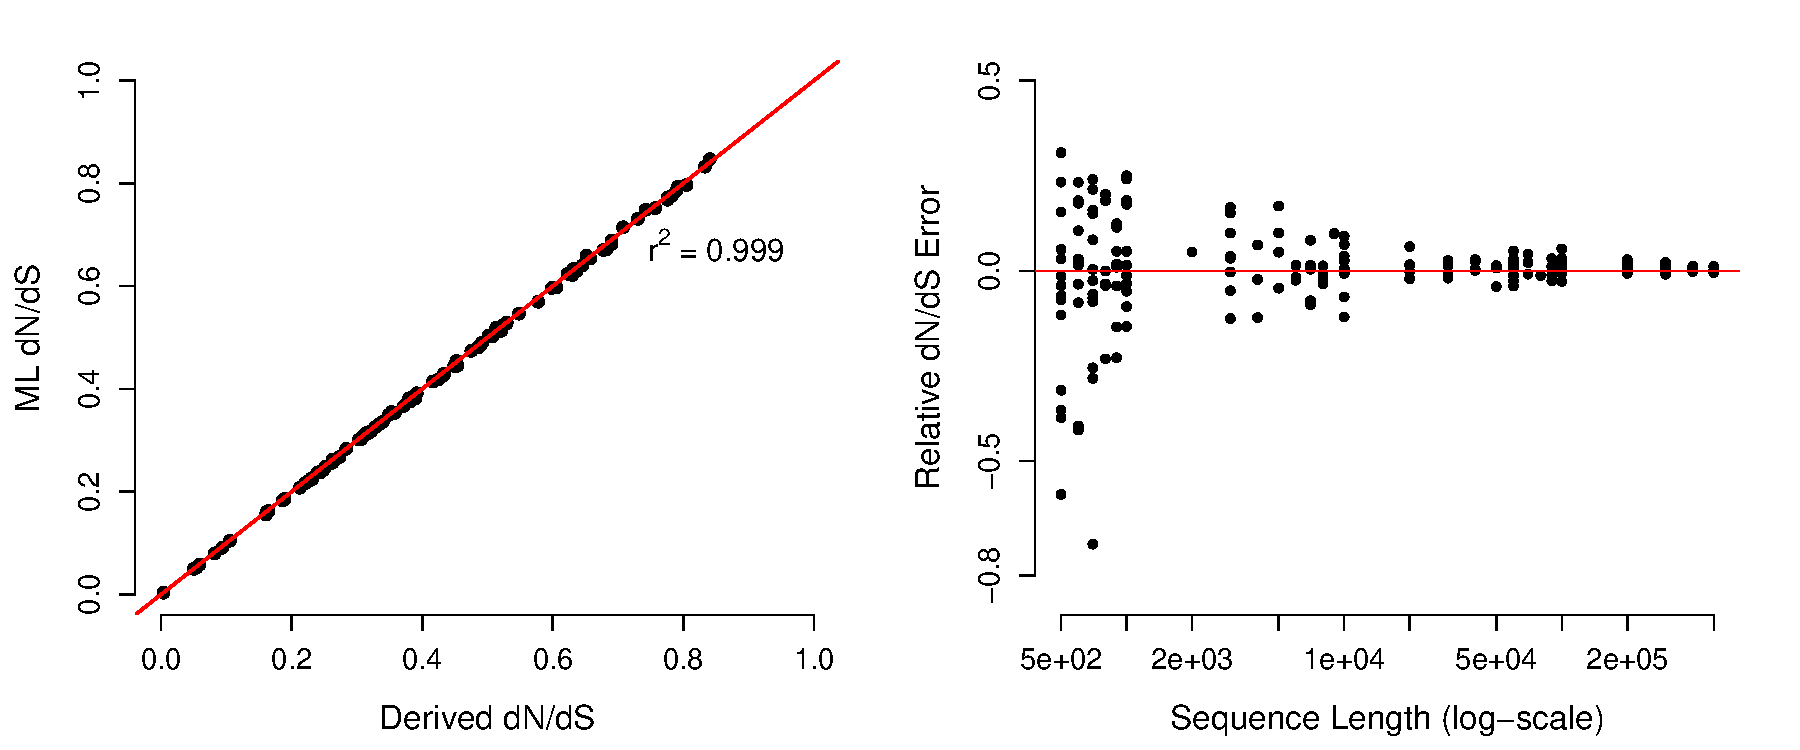
\includegraphics[width=6in]{figures/regression_convergence.pdf}}
\caption{\label{reg_conv} Relationship works exceedingly well. Left panel shows 100 points, each of which corresponds to single simulation. Note that here the ml inference is shown for equal codon frequency specs and kappa fixed to true value (a similar plot for free kappa is shown in suppfigs, but results are qualitatively identical.) Right panels shows convergence of omega values as data set size (represented as simulated alignment length) increases. The y-axis indicates relative error of the ML $dN/dS$ estimates, and the x-axis indicates sequence length on a log-scale. As the sequence length, or the data set size, increases, the two $dN/dS$ estimates converge to the same value. }
\end{figure*}

\bigskip
\begin{figure*}[H]
\centerline{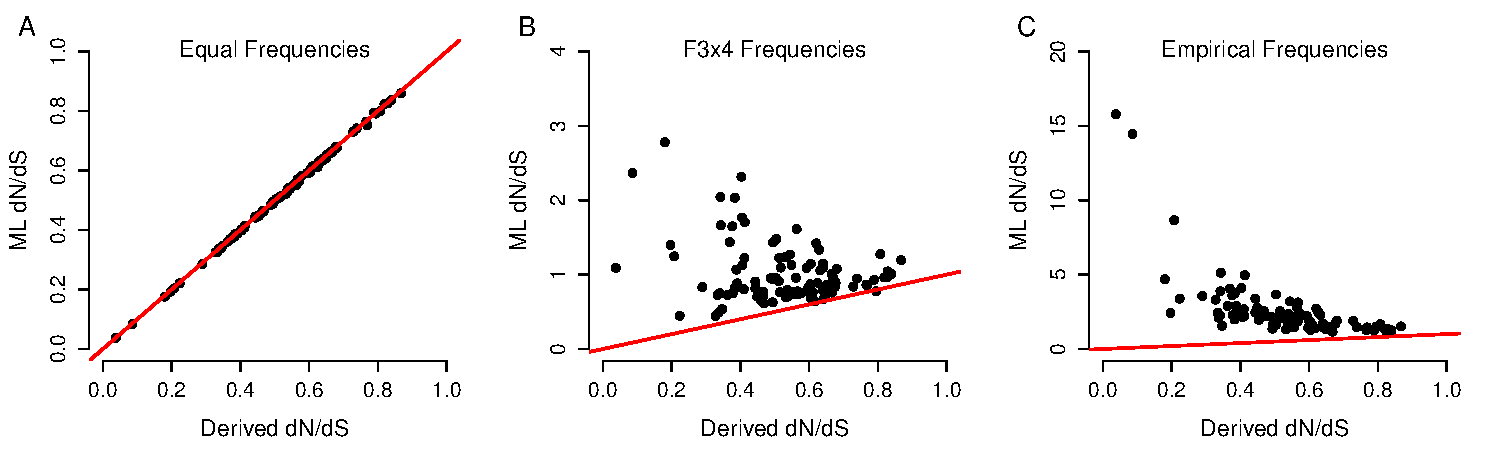
\includegraphics[width=6in]{figures/regression_fspecs.pdf}}
\caption{\label{reg_fspec} Issues with frequency specifications abound. In each plot, red line indicates 1:1 agreement, so note the y-axis differences. Relationship between omega values only really exists when equal codon frequencies are specified. When f3x4 or true freqs used, there is the potential to end up with dramatically inflated values. cf3x4 not shown because its results are statistically the same as f3x4.}
\end{figure*}

\bigskip
\begin{figure*}[H]
\centerline{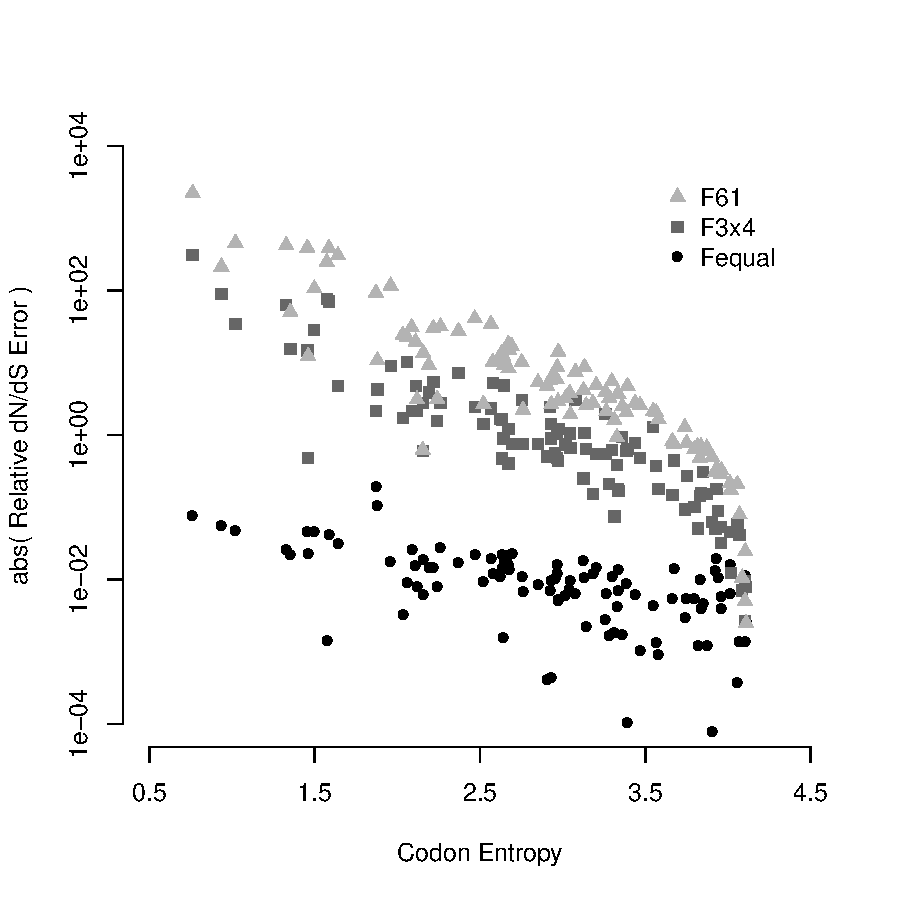
\includegraphics[width=4in]{figures/entropy_error_nobias.pdf}}
\caption{\label{entropyerror} Entropy has no independent effect here. Xaxis is data entropy, Yaxis is logscale absolute value of relative error.}
\end{figure*}



\clearpage
\newpage

\section*{Supplementary Figures and Tables}

\begin{table}[htbp]
\customlabel{tab:tabS1}{tabS1}
\begin{tabular}{c c c c c c}
\hline\noalign{\smallskip}
\multicolumn{1}{l}{Codon frequencies} & \multicolumn{1}{l}{$\kappa$ parameterization} & \multicolumn{1}{l}{$dN/dS$ correlation} &\multicolumn{1}{l}{$dN/dS$ error} & \multicolumn{1}{l}{$\kappa$ correlation} &\multicolumn{1}{l}{$\kappa$ error} \\
Equal & True & 1 & 0.008 &   &   \\ 
Equal & Free & 0.998 & 0.019 & 0.93 & 0.098 \\ 
Equal & 1 & 0.928 & 0.202 &   &   \\ 
\hline\noalign{\smallskip}
F3x4 & True & -0.053 & 1.026 &   &   \\ 
F3x4 & Free & -0.036 & 1.03 & 0.878 & 0.154 \\ 
F3x4 & 1 & 0.067 & 0.724 &   &   \\ 
\hline\noalign{\smallskip}
CF3x4 & True & -0.055 & 1.02 &   &   \\ 
CF3x4 & Free & -0.034 & 1.016 & 0.87 & 0.157 \\ 
CF3x4 & 1 & 0.056 & 0.723 &   &   \\ 
\hline\noalign{\smallskip}
Empirical & True & -0.566 & 4.735 &   &   \\ 
Empirical & Free & -0.59 & 4.728 & 0.826 & 0.206 \\ 
Empirical & 1 & -0.496 & 3.126 &   &   \\ 
\noalign{\smallskip}\hline\noalign{\smallskip}
\end{tabular}
\newline
Results from runs with codon bias. Codon frequency specifications were either set as equal (1/61 per codon), calculated from the F3x4 estimator \cite{MuseGaut1994}, calculated from the CF3x4 estimator \cite{Pond2010}, or set equal to the simulated alignment's empirical frequencies. $\kappa$ was specified as either a fixed value, its true simulated value or 1, or as a free parameter of the model. Correlations given are between the ML $\omega$ estimate and our derived $\omega$ values. Error refers to the mean absolute error between these two $\omega$ estimates. Similar values for $\kappa$ are shown for those inferences where $\kappa$ was a free parameter of the model. Note that all is significant.
\end{table}	

\clearpage


\centerline{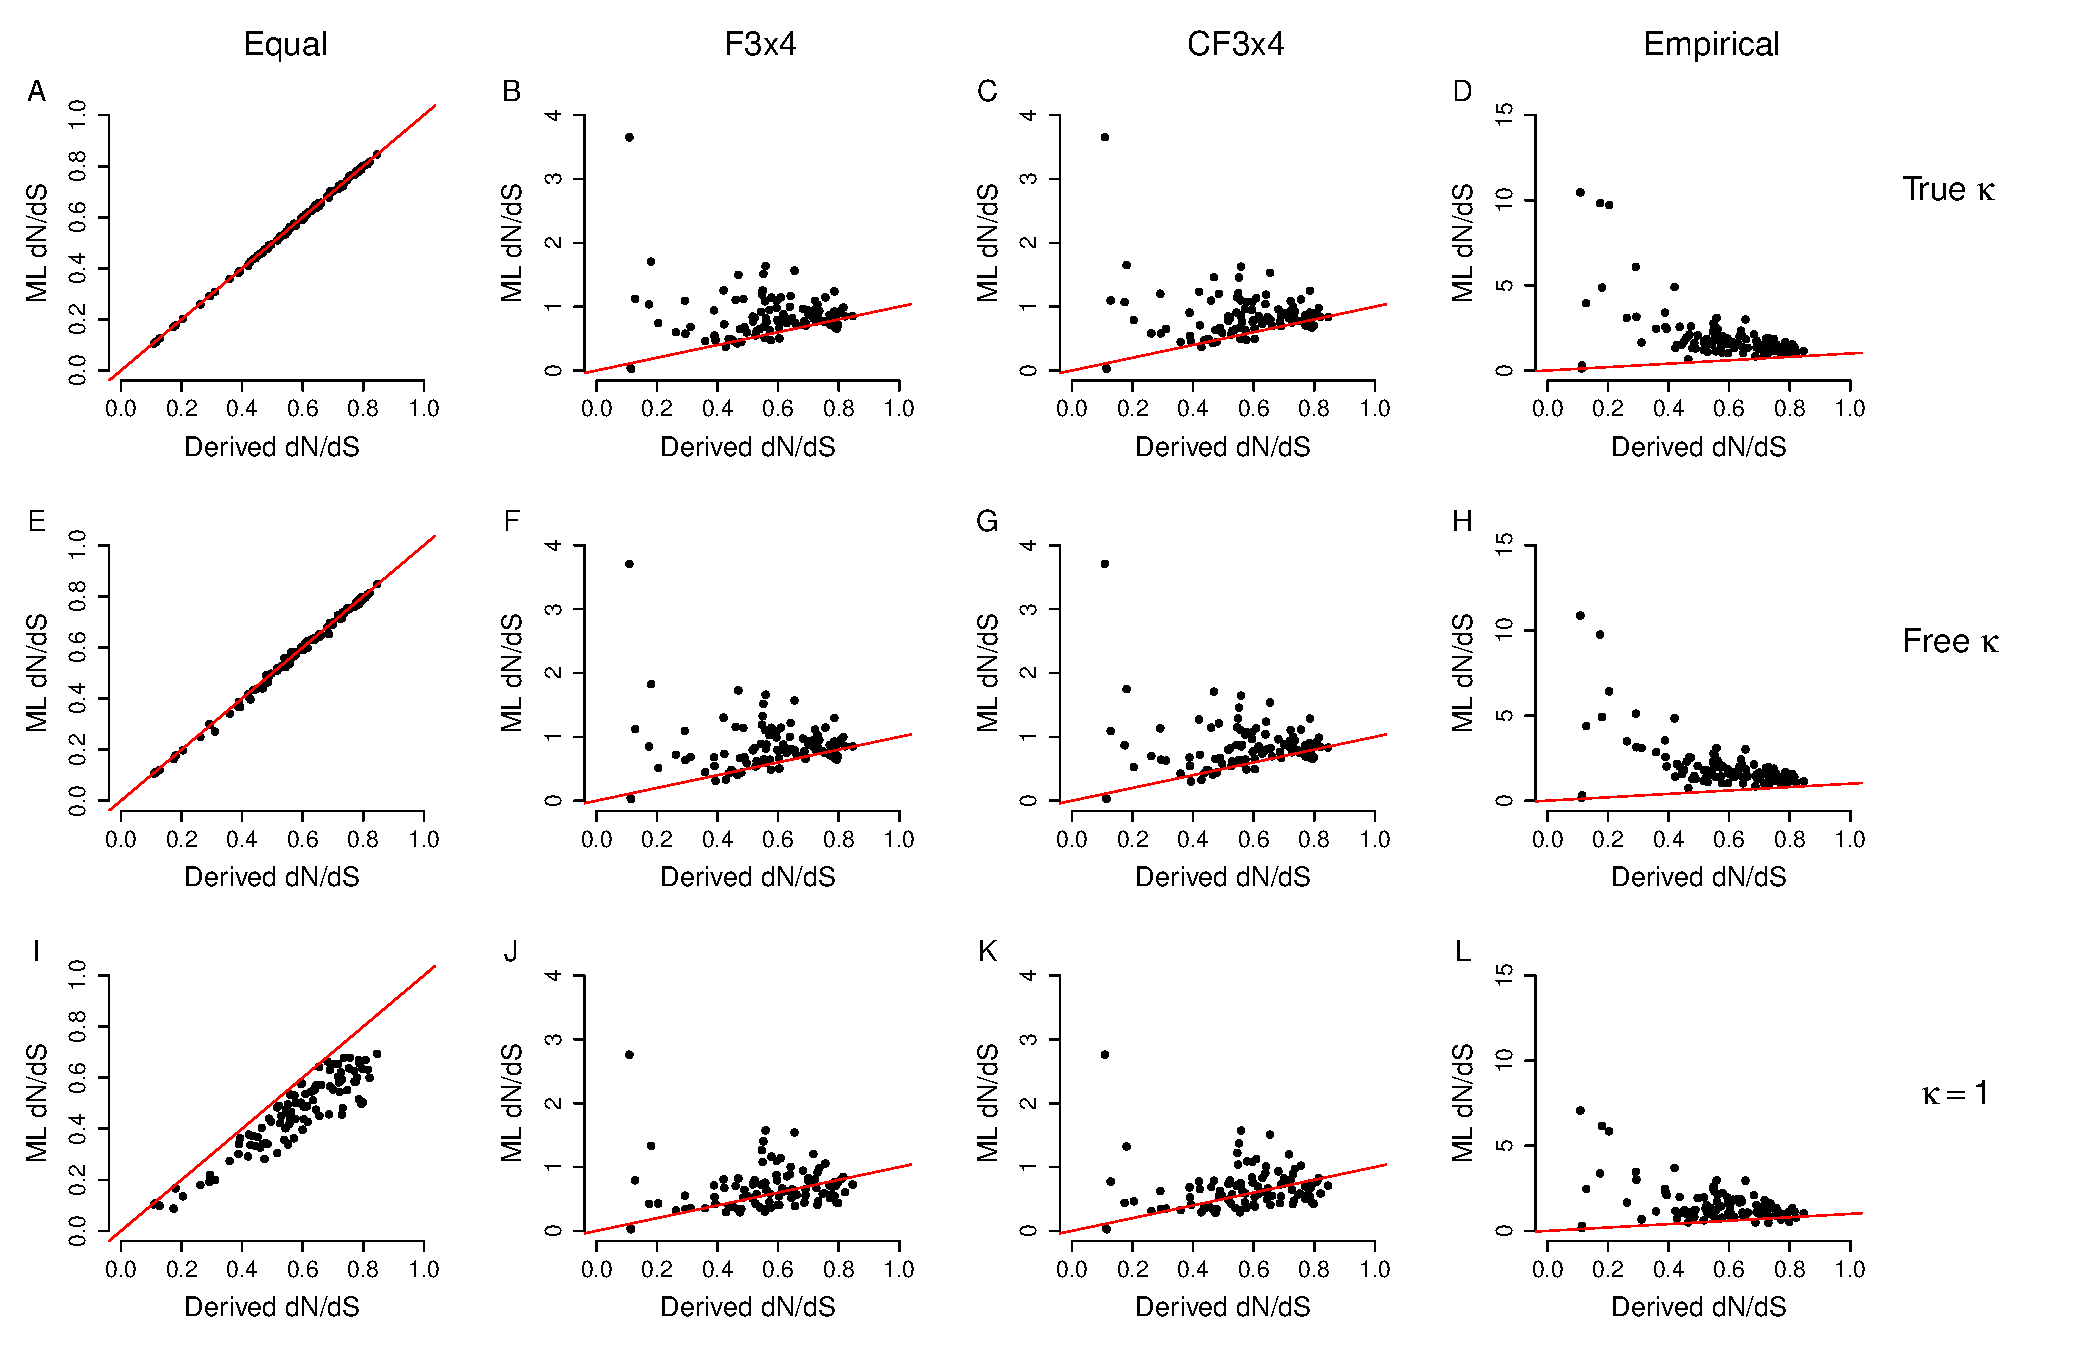
\includegraphics[width=7in]{figures/regression_allspecs_nobias.pdf}}
\noindent \textbf{Fig. S1} Omega regression for all ML parameterizations, without codon bias.
\customlabel{fig:reg_allspecs}{S1}

\clearpage


\centerline{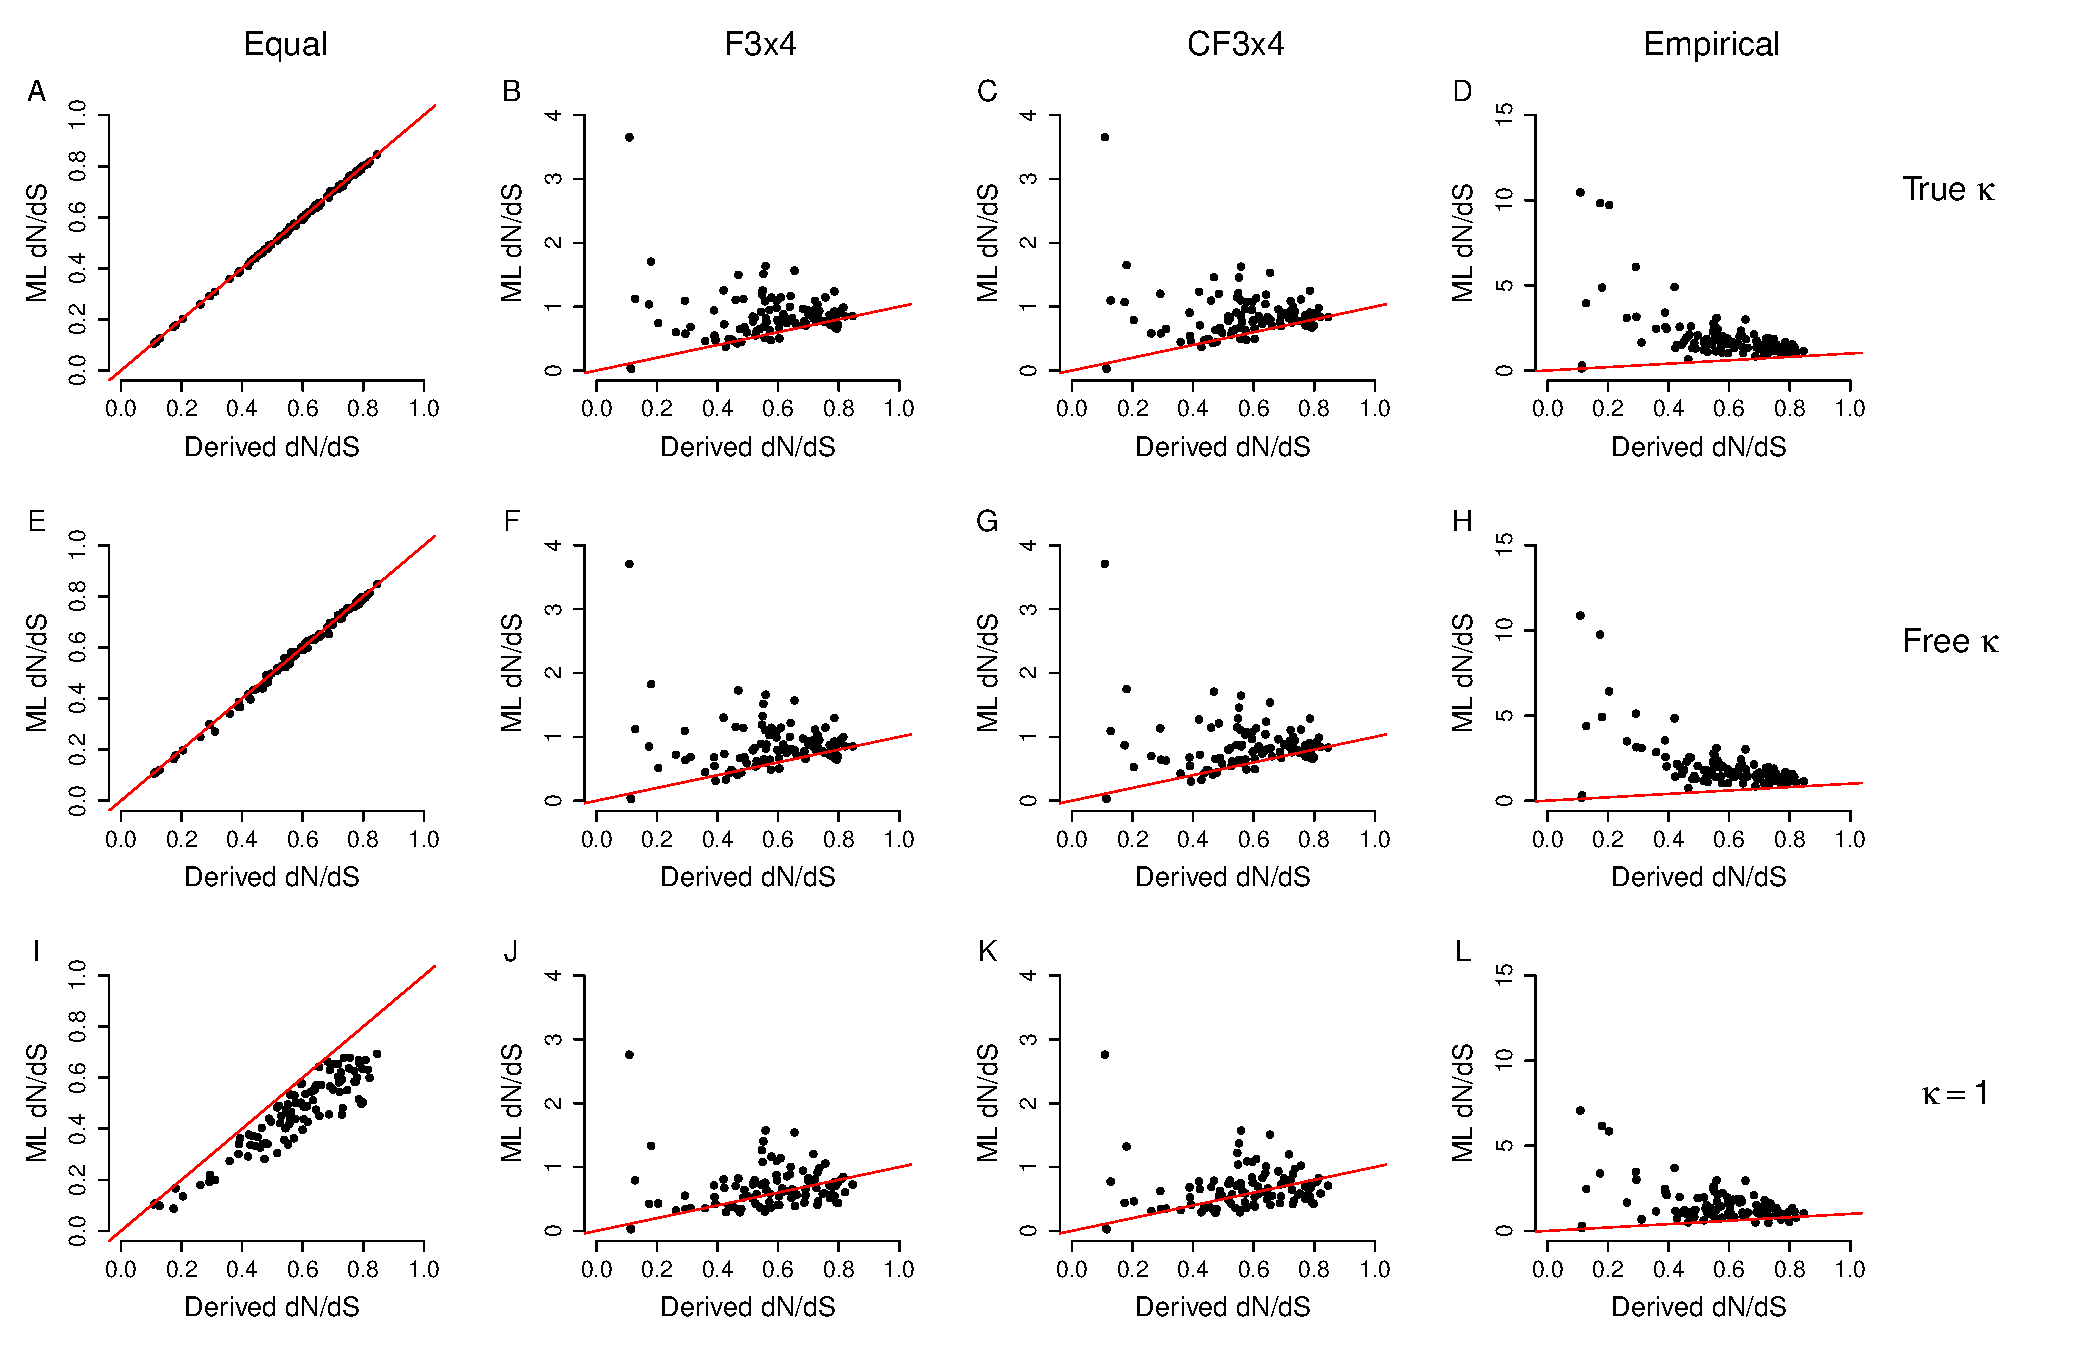
\includegraphics[width=7in]{figures/regression_allspecs_bias.pdf}}
\noindent \textbf{Fig. S2} Omega regression for all ML parameterizations, with codon bias.
\customlabel{fig:reg_allspecs}{S2}

\bigskip
\bigskip
\bigskip


\centerline{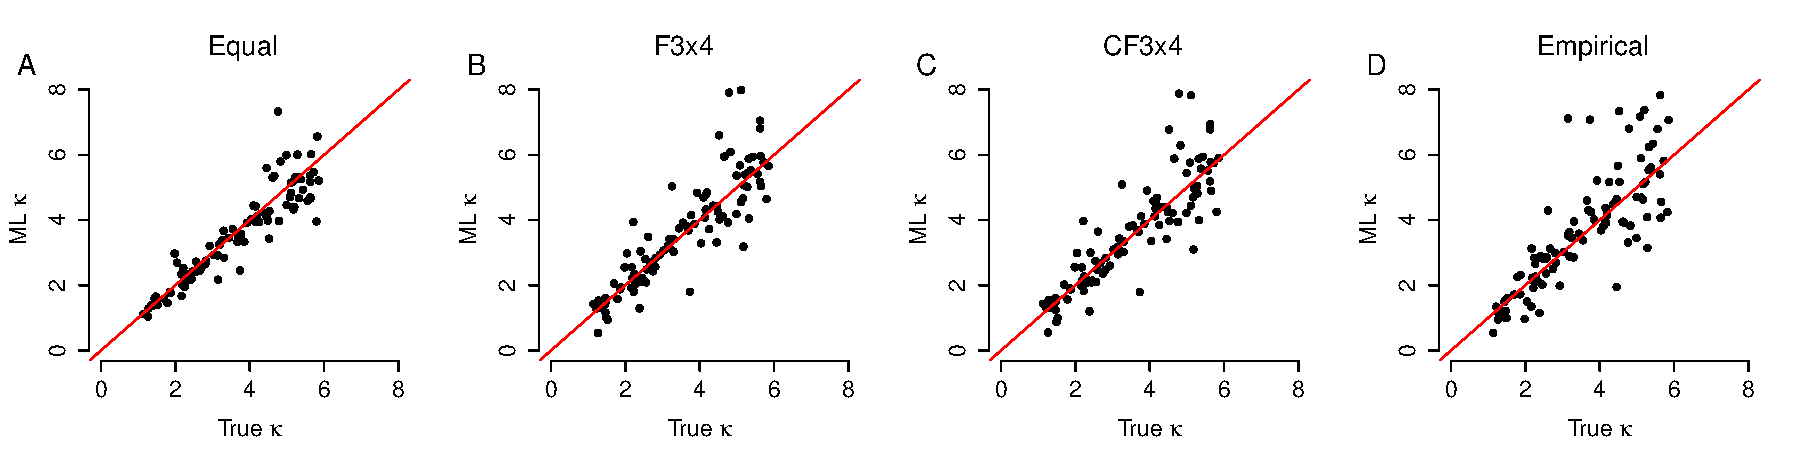
\includegraphics[width=6in]{figures/regression_kappa_nobias.pdf}}
\noindent \textbf{Fig. S3} Kappa regression for all ML freqspec parameterizations where kappa is a free parameter, without codon bias.
\customlabel{fig:reg_kappa}{S3}

\bigskip
\bigskip
\bigskip


\centerline{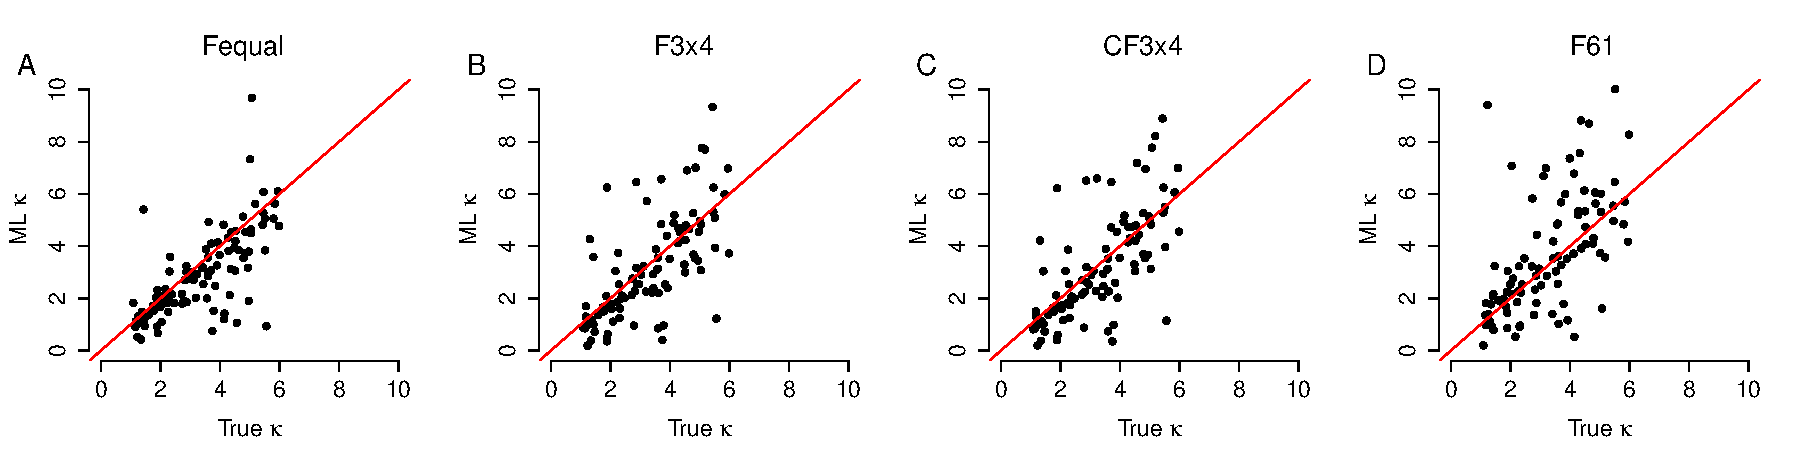
\includegraphics[width=6in]{figures/regression_kappa_bias.pdf}}
\noindent \textbf{Fig. S4} Kappa regression for all ML freqspec parameterizations where kappa is a free parameter, without codon bias.
\customlabel{fig:reg_kappa}{S4}

\clearpage

\centerline{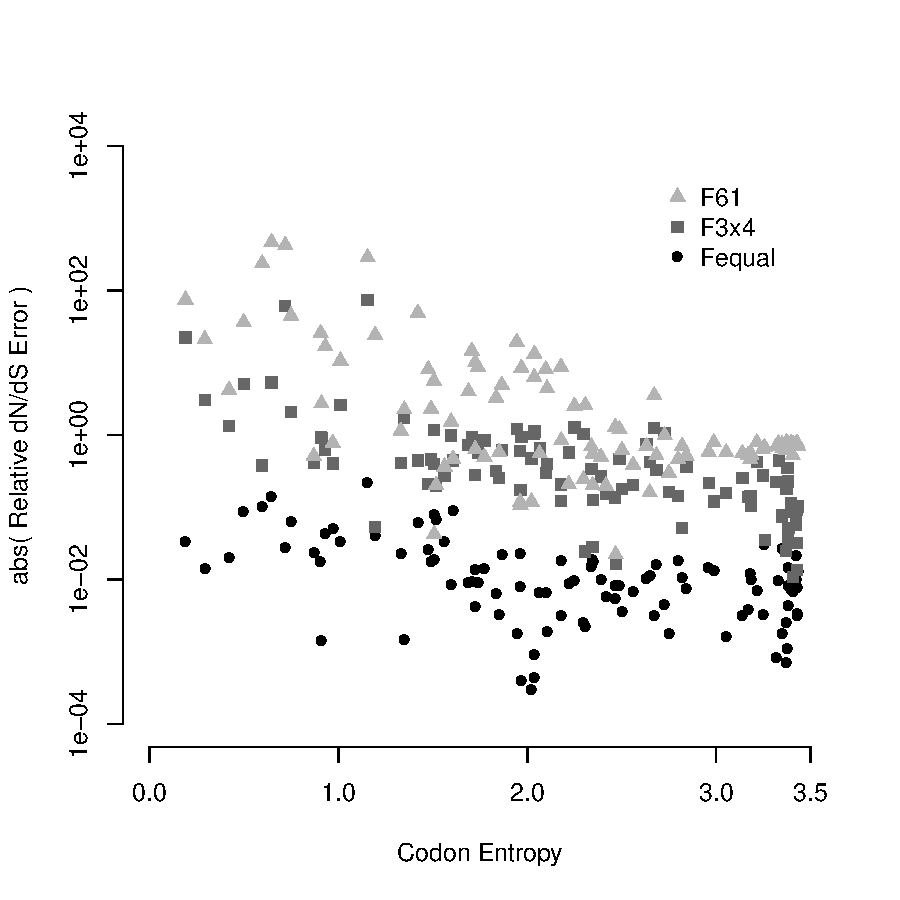
\includegraphics[width=4in]{figures/entropy_error_bias.pdf}}
\noindent \textbf{Fig. S5} Entropy and error for the codon bias data set.
\customlabel{fig:reg_kappa}{S5}

\end{document}

